\RequirePackage{silence} % :-\
    \WarningFilter{scrbook}{Usage of package `titlesec'}
    \WarningFilter{titlesec}{Non standard sectioning command detected}
\documentclass[11pt,paper=b5,footinclude,headinclude]{scrbook} % KOMA-Script book
\usepackage[T1]{fontenc}
\usepackage[style=arsclassica, parts=false, eulermath=false, palatino=true, eulerchapternumbers=true]{classicthesis}

\usepackage{afterpage}
\usepackage{xcolor}
\usepackage{xspace}
\usepackage{etoolbox}
\providetoggle{long}


%framed example
\usepackage[framemethod=TikZ]{mdframed}
% EXAMPLES
%% set the counter for your environment
\newcounter{example}
\renewcommand{\theexample}{\thechapter.\arabic{example}}

%% define the style
\mdfdefinestyle{example}{%
    linecolor=blue,
    backgroundcolor=blue!5,
    outerlinewidth=2pt,
    bottomline=false,
    leftline=false,rightline=false,
    skipabove=\baselineskip,
    skipbelow=\baselineskip,
    frametitle=\mbox{},
}
%% setup the environments
%%% with number
\newmdenv[%
    style=example,
    settings={\global\refstepcounter{example}},
    frametitlefont={\bfseries Zgled~\theexample\quad},
]{example}
%%% without number (starred version)
\newmdenv[%
    style=example,
    frametitlefont={\bfseries Zgled~\quad},
]{example*}



\newcommand{\komentar}[1]{\textcolor{red}{[#1]}} %for displaying red texts

\usepackage{fullpage}
%\usepackage{fancyhdr}
\usepackage{enumerate}


\usepackage[slovene]{babel} % slovenske nastavitve (naslovi, deljenje besed ...)
\usepackage[utf8]{inputenc}
\usepackage{amsfonts,amssymb}
\usepackage{graphicx}
\usepackage{amsmath,amssymb,amsthm}
\usepackage{epsf}
\usepackage{epsfig}
\usepackage{graphics}
\usepackage{color}
\usepackage{comment}
%\usepackage{times}
%\usepackage{txfonts}
\def\P {{\cal P}}
\def\ali {{~\vee~}}
\def\inn {{~\wedge~}}
\def\sledi {{~\Rightarrow~}}
\def\brez {{\,\setminus\,}}
\def\cee {{~\Leftrightarrow~}}
\def\zgled{\noindent\textbf{\color{blue} Zgled: }}
\def\kz{{\hfill{\color{blue}$\blacktriangle$}}}% konec zgleda
%\parskip=7pt
%
%\textwidth=17cm\textheight=22cm\parindent=15pt\parskip=5pt
%\oddsidemargin=-5mm  \headheight=0pt \pagestyle{plain}

%spremenljivke
\newcommand{\myTitle}{Teoretične osnove računalništva\xspace}
\newcommand{\mySubtitle}{Diskretne strukture za računalničarje \xspace} 				%dodaj podnaslov if needed
\newcommand{\myName}{UP FAMNIT \xspace}
\newcommand{\myPublisher}{XXX}
\newcommand{\myMonth}{Pomlad}
\newcommand{\myYear}{2021}
\newcommand{\verzija}{Verzija 0.1 }

\newcommand{\frontpageAuthors}{Matjaž Krnc}
\newcommand{\myRepo}{\url{https://github.com/mkrnc/TOR1-vaje---TCS1-exercises.git}}


\newcommand{\shortAuthors}{M. Krnc}
\newcommand{\myAuthors}{Matjaž Krnc}


\newcommand{\myISBN}{978-961-XXX-XXX-X }


\newtheorem*{trditev}{Trditev}
\newtheorem*{izrek}{Izrek}
\newtheorem*{problem}{Naloga}
\newtheorem*{lema}{Lema}
\newtheorem*{posledica}{Posledica}
\newtheorem*{definicija}{Definicija}
\newtheorem*{zg}{Zgled}


\begin{document}
%*******************************************************
% Titlepage
%*******************************************************
\begin{titlepage}
\definecolor{amber}{rgb}{1.0, 0.75, 0.0}
\pagecolor{amber}\afterpage{\nopagecolor}
	% if you want the titlepage to be centered, uncomment and fine-tune the line below (KOMA classes environment)
	\begin{addmargin}[-1cm]{-1cm}
    \begin{center}
        \large  

        \hfill

        \vfill

        \begingroup
            \color{Maroon}\spacedallcaps{\LARGE\myTitle} \\ \bigskip
        \endgroup

        \spacedlowsmallcaps{\mySubtitle}

        \vfill

        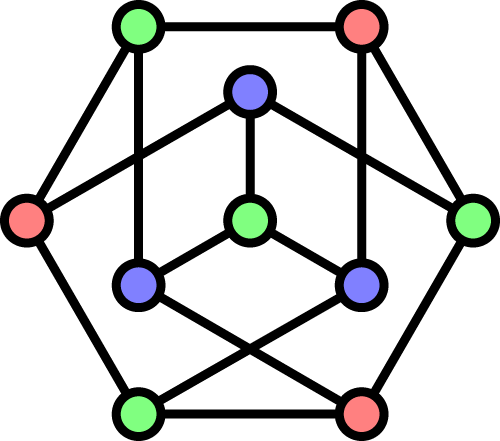
\includegraphics[width=11cm]{petersen.png} %\\ \medskip
				\vfill
        \myName \\ \medskip   
        %\myDegree \\
        %\myDepartment \\                            
        %\myFaculty \\
        %\myUni \\ \bigskip

        \myMonth \xspace \myYear \ -- \verzija

        \vfill                      

    \end{center}  
  \end{addmargin}       
\end{titlepage}   

%\begin{addmargin}[-1cm]{-1cm}
	{\vspace*{\fill}
	\setlength{\fboxsep}{6mm}
	\noindent\fbox{
	\begin{minipage}[b][6.5cm][c]{11cm} % velikost okvira škatle je 11 cm
							% x 6,5 cm
	\small
	CIP -- Katalo\v zni zapis o publikaciji\\
	Narodna in univerzitetna knji\v znica, Ljubljana
	
	\vfill

	123.4(567)(8.901.2)
	\vfill

	TEORETIČNE osnove računalništva [Elektronski vir] : Diskretne strukture za računalničarje / avtorji \shortAuthors; [urednik] M. Krnc. - Verzija \myVersion.  - El. knjiga. - Ljubljana : samozal. M. Krnc, 2020.
	\vfill
	
	Način dostopa (URL):\\ \url{https://github.com/mkrnc/TOR1-zapiski-s-predavanj}
	
	\vfill
	
	ISBN \myISBN  (pdf)\\
	%1. Milanič, Martin 2. Krnc, Matjaž, 1987-
	123456789
	\vfill
	
	\end{minipage}}}
%\end{addmargin}
\endinput
\newpage
\section*{Predgovor}
Pred tabo so zapiski iz predavanj za predmet TOR1, ki se predava študentom prvega letnika na FAMNIT, Univerza na Primorskem.
Predmet pokriva osnove iz različnih področij teoretičnega računalništva in je usmerjen potrebam računalničarjev.
%Od leta 2020 naprej sem se odločil tale TeX projekt odpreti kot javni repozitorij, tako da lahko zares vsak študent predlaga svoje naloge (oz. rešitve), ki se jih ustrezno vključi v tole skripto.


Dokument je zamišljen kot dopolnjevanje predavanj, in se ga ne sme jemati kot samostojno gradivo za pripravo na izpit. 
Morebitna vprašanja in najdene napake, lepo prosim, sporočite na
\url{matjaz.krnc@upr.si}, oz. ustvarite t.i. "issue"\xspace na našem javnem repozitoriju.
\begin{center}
    \url{https://github.com/mkrnc/TCS1-course-notes.git}.    
\end{center}


%Among most notable student contributors are:

\newpage
\vspace*{\fill}
\noindent

\begin{tabular}{ll}
%Lektorirala: ...\\[3mm]
\multicolumn{2}{ l }{\textbf{\myTitle}} \\
\multicolumn{2}{ l }{\emph{\mySubtitle}} \\[6mm]
\textbf{Avtor:} & \parbox[t]{6cm}{\myAuthors \vspace{3mm}}\\
\textbf{Samozaložba in oblikovanje:} & Matjaž Krnc\\[3mm]
%E-po�ta: knjiga@vidra.net\\[3mm]
%Za zalo�bo: Andrej Klemenc\\[3mm]
%\textbf{Oblikovanje:} & Matjaž Krnc\\[3mm]
\textbf{ISBN:} &  \myISBN \\
%Priprava za tisk: \\[3mm]
%Tisk: \\[3mm]
Ljubljana, \myMonth\xspace\myYear
\end{tabular}
\endinput

\tableofcontents


\chapter{Matematična logika}

\begin{enumerate}
\item Dani sta izjavi $A$: "Zunaj je mrzlo." in $B$: "Zunaj dežuje.". V naravnem jeziku napiši naslednje sestavljene izjave:
\begin{enumerate}
  \item $\neg A$
  \item $A \land B$
  \item $A \lor B$
  \item $B \lor \neg A$
\end{enumerate}

\item Naj bo $A$: "Janez bere Finance.", $B$: "Janez bere Delo.", in $C$: "Janez bere Večer.".
Prepiši v simbolne izjave:
\begin{enumerate}
  \item Janez bere Finance ali Delo, a ne Večera. \[(A \lor B) \land \neg C\]
  \item Janez bere Finance in Delo ali pa ne bere Financ in Dela. \[(A \land B) \lor \neg (A \land B)\]
  \item Ni res, da Janez bere Finance, ne pa Večera. \[\neg (A \land \neg C)\]
  \item Ni res, da Janez bere Večer ali Delo, ne pa Financ. \[\neg ((B \lor C) \land \neg A)\]
\end{enumerate}

\item Poišči pravilnostne tabele za primere v prejšnji nalogi.

\item Za tri različne premice $p$, $q$ in $r$ v prostoru velja $(p \parallel r) \land (p \cap q = A) \land (q \cap r = B)$. Kaj lahko sklepaš? Rešitev: Nariši skico. Premica $q$ leži v ravnini, in jo določata $p$ in $r$.

\item Vitezi in oprode (vitez vedno govori resnico, oproda vedno lažejo):
\begin{enumerate}
  \item Artur: Ni res, da je Cene oproda.
  Bine: Cene je vitez ali pa sem jaz vitez.
  Cene: Bine je oproda.
  Kdo od njih je vitez in kdo oproda?
  \item Artur: Cene je oproda ali je Bine oproda.
  Bine: Cene je vitez in Artur je vitez.
  Kdo od njih je vitez in kdo oproda?
\end{enumerate}

\item Z osnovnima povezavama $\neg$ in $\land$ izrazi naslednje sestavljene izjave:
\begin{enumerate}
  \item $A \lor B$
  \item $A \rightarrow B$
  \item $A \iff B$
\end{enumerate}

\item Prepričaj se, da veljajo naslednje logične ekvivalence:
\begin{enumerate}
  \item $A \land (B \lor C) \iff \neg (A \land B) \rightarrow (A \land C)$
  \item $\neg A \land (A \rightarrow B) \iff A \rightarrow (\neg A \land B)$
  \item $A \lor B \lor C \iff \neg (A \lor B) \rightarrow C$
  \item $(A \rightarrow B) \land (B \rightarrow A) \iff (A \land B) \lor (\neg A \land \neg B)$
\end{enumerate}

    \item 
    (Naloga o vitezih in oprodah)
A, B, C, D, E
\begin{itemize}
  \item A: ``D je oproda in C je oproda."
  \item B: ``Če sta A in D oprodi, potem je C oproda."
  \item C: ``Če je B oproda, potem je A vitez."
  \item D: ``Če je E oproda, potem sta C in B oprodi."
\end{itemize}

\medskip
\textbf{Rešitev:}

Naj bo $A$ izjava: ``A je vitez", itd.
Iščemo tisto edino določilo $d$, za katerega je izjava $$A_1\inn B_1\inn C_1\inn D_1$$
pravilna, kjer je:

$A_1: A\cee (\neg D \inn \neg C)$

$B_1: B\cee (\neg A \inn \neg D\sledi \neg C)$

$C_1: C\cee (\neg B \sledi A)$

$D_1: D\cee (\neg E \sledi \neg C \inn \neg B)$


Ker bi pravilnostna tabela vsebovala 32 vrstic, rešimo nalogo
raje z analizo primerov.

\textbf{1.~primer: $A(d) = 1$.}
Zaradi $A_1$ je potem $D(d) = 0$ in $C(d) = 0$.

V izjavo $C_1$ vstavimo $A(d) = 1$ in $C(d) = 0$, dobimo:
$\neg(\neg B\sledi 1)$,

$\neg(B\ali 1)$,

$\neg 1$, to pa je nepravilna izjava.

Torej 1.~primer ni mogoč.
%
% torej $B(d) = 1$.
%
%V izjavo $B_1$ vstavimo $A(d) = 1$, $B(d) = 1$, $C(d) = 0$ in $D(d) = 0$, dobimo:
%$1\cee (0\inn 1\sledi 1)$, kar je pravilna izjava.
%
%V izjavo $D_1$ vstavimo znane vrednosti, dobimo:
%$\neg(\neg E \sledi 1 \inn 0)$
%
%$\neg(\neg E \sledi 0)$
%
%Sledi $\neg E(d) = 1$, torej $E(d) = 0$.
%

\textbf{2.~primer: $A(d) = 0$.}

Zaradi $A_1$ je bodisi $C(d) = 1$ ali pa $D(d) = 1$.

\textbf{2.1.: $C(d) = 1$}.

Zaradi $C_1$ je $\neg B \sledi 0$, torej je $\neg B = 0$ in posledično $B(d) = 1$.

V izjavo $B_1$ vstavimo $A(d) = 0$, $B(d) = 1$, $C(d) = 1$, dobimo:

$1 \inn \neg D\sledi 0$

$\neg D\sledi 0$

Sledi $\neg D = 0$ oz.~$D(d) = 1$.

Vstavimo v izjavo $D_1$ znane vrednosti:

$(\neg E \sledi 0 \inn 0)$

Sledi $E(d) = 1$.

\bigskip

\textbf{2.2.: $C(d) = 0$ in $D(d) = 1$}.

Iz izjave $B_1$ dobimo $B(d) = 1$.

Izjava $C_1$ pa je sedaj nepravilna:
$0 \cee (0\sledi 1)$.\qed

Torej so $B$, $C$, $D$ in $E$ vitezi, $A$ pa je oproda.


\bigskip
\item (Sklepanje)
Ali je naslednje sklepanje pravilno?

Mislim, torej sem. Mislim, torej sklepam. Sklep: Sem, torej sklepam.


\textbf{Rešitev:}

$A_1$: Mislim.

$A_2$: Sem.

$A_3$: Sklepam.

Zanima nas pravilnost implikacije

$$(A_1\sledi A_2)\inn(A_1\sledi A_3)\sledi(A_2\sledi A_3)$$

Pri določilu $A_1(d) = 0$, $A_2(d) = 1$, $A_3(d) = 0$ je ta implikacija nepravilna!
(Ne mislim, sem, ne sklepam.)
Torej je sklepanje napačno.

\bigskip

\item (Sklepanje)
Ali je naslednje sklepanje pravilno?

Dojenčki se obnašajo nelogično. Kdor je sposoben ukrotiti krokodila, je spoštovanja vreden.
Kdor se obnaša nelogično, ni spoštovanja vreden. Sklep: Dojenčki niso sposobni ukrotiti krokodila.


\textbf{Rešitev:}

$A_1$: Sem dojenček.

$A_2$: Obnašam se nelogično.

$A_3$: Sposoben sem ukrotiti krokodila.

$A_4$: Vreden sem spoštovanja.

$(A_1\sledi A_2)\inn (A_3\sledi A_4) \inn (A_2\sledi \neg A_4)\sledi (A_1\sledi \neg A_3)$

Pa recimo, da je sklep napačen. Tedaj obstaja določilo $d$, da velja
\begin{enumerate}[(1)]
  \item $(A_1(d)\sledi \neg A_3(d)) = 0$
  \item $(A_1(d)\sledi A_2(d)) = 1$
  \item $(A_3(d)\sledi A_4(d)) = 1$
  \item $(A_2(d)\sledi \neg A_4(d)) = 1$
\end{enumerate}
Torej je, zaradi (1), $A_1(d) = 1$ in $A_3(d) = 1$. Zaradi (2) je $A_2(d) = 1$.
Zaradi (4) je $A_4(d) = 0$. To pa je protislovje s (3).

Torej je sklepanje pravilno.\qed

% 8. in 9. predavanje, 4 ure (Istvan), 7. in 8. 11. 2012

%\bigskip
%Rešitev domače naloge:
%
%Dejstva:
%
%Barona je umoril eden izmed njegovega osebja: kuharica, strežnik ali šofer.
%
%Če je morilka kuharica, je zastrupila hrano.
%
%Če je morilec šofer, mu je postavil bombo v avto.
%
%Hrana ni bila zastrupljena in strežnik ni morilec.
%
%Sklep: Morilec je šofer.
%
%\bigskip
%
%\textbf{ Rešitev:}
%
%$K$: Morilka je kuharica.
%
%$S$: Morilec je strežnik.
%
%Š: Morilec je šofer.
%
%H: Kuharica je zastrupila hrano.
%
%B: Šofer je postavil bombo v avto.
%
%\medskip
%Ali je naslednja implikacija tavtologija?
%
%$(K\ali S\ali$ \v S$)\inn(K\sledi H)\inn($Š$\sledi B)\inn(\neg H\inn \neg S)\sledi $Š
%
%\bigskip
%Recimo, da ni.
%
%(1) $(K\ali S\ali$ \v S$)(d) = 1$
%
%(2) $(K\sledi H)(d) = 1$
%
%(3) (Š$\sledi B)(d) = 1$
%
%(4) $(\neg H\inn \neg S)(d) = 1$
%
%(5) Š$(d) = 0$
%
%Iz (4) sledi:
%
%(5)  $H(d) = S(d) = 0$.
%
%Iz (2) in (5) potem sledi
%
%(6) $K(d) = 0$.
%
%Iz (1), (5) in (6) potem sledi Š$(d) = 1$. Protislovje. Izjava je tavtologija  in sklepanje je pravilno.
%


\item
The following two propositions are given:
$A$: ``Andrej speaks French.'' and $B$: ``Andrej speaks Danish.''
Write the following compound propositions in natural language:

(a) $A\ali B$

(b) $A\inn B$

(c) $A\inn \neg B$

(d) $\neg A\ali \neg B$

(e) $\neg \neg A$

(f) $\neg (\neg A\inn \neg B)$

\medskip
\item
The following two propositions are given:
$A$: ``Janez is rich.'' and $B$: ``Janez is happy.''

Write the following propositions symbolically:

(a) If Janez is rich, then he is unhappy.

(b) Janez is neither happy nor rich.

(c) Janez is happy only if he is poor.

(d) Janez is poor if and only if he is unhappy.

\item Solve the following exercises about knights and servants:
\begin{itemize}
  \item Arthur: ``It is not true that Bine is a servant."~Bine: ``We are not both of the same kind.''
  \item Arthur: ``It is not true that Cene is servant."~Bine: ``Cene is a knight or I am a knight."~Cene: ``Bine is a servant."
\end{itemize}

\item {A similar exercise:}
Now Arthur and Bine say the following:
\begin{itemize}
 \item Arthur: ``Me and Bine are not of the same kind.''
 \item Bine: ``Exactly one of us is a knight.''
\end{itemize}
\item Given the propositions:\\
$A:$ ``It's cold outside''\\
$B:$ ``It's raining''\\
express the following propositions in natural language:
\begin{enumerate}
\item $\neg A$
\item $A\wedge B$
\item $A\vee B$
\item $B\vee\neg A$
\end{enumerate}
\item Given the propositions:\\
$A:$ ``John reads The New York Times.''\\
$B:$ ``John reads The Wall Street Journal.''\\
$C:$ ``John reads The Daily Mail.''\\
\\
Transcribe the following statements into symbolic propositions:
\begin{enumerate}
\item John reads The New York Times, but not The Wall Street Journal.
\item Either John reads both The New York Times and The Wall Street Journal,
or he does not read The New York Times and The Wall Street Journal.
\item It is not true that John reads The New York Times, and does not read
The Daily Mail.
\item It is not true that John reads The Daily Mail or The Wall Street Journal,
and not The New York Times.
\end{enumerate}
\item Find the truth tables for the symbolic propositions from (2).
\begin{enumerate}
\item For three lines $p,q,r$ we may construct also geometric propositions.
Suppose that the following is true:
\[
(p||q)\wedge(p\cap q\neq\emptyset)\wedge(q\cap r\neq\emptyset).
\]
What can you ay about the lines $p,q,r$?
\end{enumerate}
\item Knights and servants! For both cases below (separately) determine
the roles.
\begin{enumerate}
\item Arthur: It's not true that Chloe is a servant.\\
Bob: Chloe is a knight, or I am a knight.\\
Chloe: Bob is a servant.
\item Arthur: Chloe or Bob are servants.\\
Bob: Cene and Arthur are knights.
\end{enumerate}
\item Express the propositions below with connectives $\wedge$ and $\neg$
only!
\begin{enumerate}
\item $A\vee B$
\item $A\Rightarrow B$
\item $A\Leftrightarrow B$
\end{enumerate}


\item Find the canonical disjunctive normal form (DNF) and the canonical conjuctive normal form (CNF) for the following propositions:
\begin{enumerate}
\item[(i)] $\neg(A\wedge B) \Rightarrow (\neg B \Rightarrow A)$
\item[(ii)] $\neg (A\vee B) \wedge (A \Rightarrow B)$
\end{enumerate}

\emph{Re"sitev.} (i) Napi"si pravilnostno tabelo. DNO: vzemi vrstice z enicami (pove"zi jih med sabo s konjunkcijo) in jih pove"zi med sabo z disjunkcijo
$(A\wedge B) \vee (A\wedge \neg B) \vee (\neg A \wedge B)$. KNO: vzemi vrstice z ni"clami (vzemi nasprotne vrednosti in jih pove"zi med sabo z disjunkcijo) in jih pove"zi med sabo s konjunkcijo $(A \vee B)$. (ii) Podobno.

\item For the following compound proposition find  a truth table, determine DNF, CNF and draw the corresponding circuit.
$$
(A \Rightarrow (B\Rightarrow C)) \Rightarrow ((A\Rightarrow B)\Rightarrow (A \Rightarrow C)).
$$


\item Find a compound proposition $\mathcal{I}$ such that
$$(A\Rightarrow (\mathcal{I} \Rightarrow \neg B))\Rightarrow (A\wedge B) \vee \mathcal{I}$$
is tautology.

\emph{Re"sitev.} Napi"si pravilnostno tabelo za osnovni izjave $A, B$ skupaj s (sestavljeno) izjavo $\mathcal{I}$. Iz nje razberi, da je pravilnostna tabela za $\mathcal{I}$ enaka
\begin{table}[ht!]
\centering
\begin{tabular}{c|c|c}
A & B & $\mathcal{I}$\\
\hline
1 & 1 & 0\\
1 & 0 & 1\\
0 & 1 & 1\\
0 & 0 & 1
\end{tabular}
\end{table}

Torej je $\mathcal{I} \Leftrightarrow \neg A \vee \neg B$ v KNO.
\pagebreak

\item For the following circuits find the  corresponding compound propositions

\noindent (i)
\begin{center}
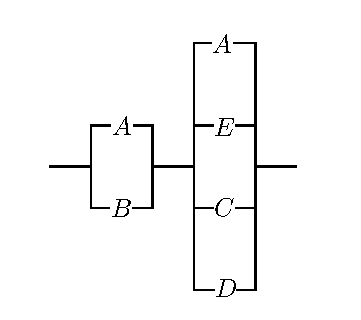
\includegraphics{img/vez1}
\end{center}
\noindent (ii)
\begin{center}
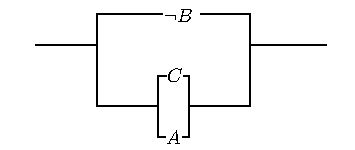
\includegraphics{img/vez2}
\end{center}
\noindent (iii)
\begin{center}
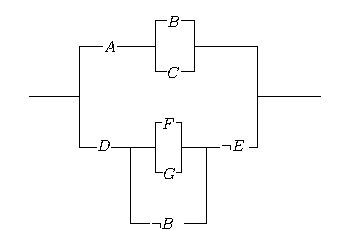
\includegraphics{img/vez3}
\end{center}




\item Simplify the following logical equivalence
$$(A\Rightarrow B) \vee (B \Rightarrow C).$$

\emph{Re"sitev.} 
\begin{eqnarray*}
(A\Rightarrow B) \vee (B \Rightarrow C) &\Leftrightarrow & (\neg A \vee B) \vee (\neg B \vee C)\\
&\Leftrightarrow & \neg A \vee B \vee \neg B \vee C\\
&\Leftrightarrow & \neg A \vee (B \vee \neg B) \vee C\\
&\Leftrightarrow & \neg A \vee 1 \vee C\\
&\Leftrightarrow & 1.
\end{eqnarray*}

\item Show that the following propositions are logical implications (a tautology where the main connective is implication).
\begin{enumerate}
\item[(i)] $A \wedge (A \Rightarrow B) \Rightarrow B$
\item[(ii)] $\neg B \wedge (A \Rightarrow B) \Rightarrow \neg A$
\item[(iii)] $\neg A \wedge (A \vee B) \Rightarrow B$
\item[(iv)] $(A \Rightarrow B) \wedge (B \Rightarrow C) \Rightarrow (A \Rightarrow C)$
\item[(v)] $A \wedge (A \Leftrightarrow B) \Rightarrow B$
\end{enumerate}

\emph{Re"sitev.} (i) Recimo $A \wedge (A \Rightarrow B)$ pravilna, $B$ pa nepravilna. Potem je $A$ pravilna in $A\Rightarrow B$ pravilna. Sledi $B$ pravilna. Protislovje. 


\item Are the following propositions logical implications?
\begin{enumerate}
\item[(i)] $(A \Rightarrow B ) \wedge (A \Rightarrow C) \wedge A \Rightarrow B \wedge C$
\item[(ii)] $\neg (A \vee B) \wedge (A\vee C) \wedge (D\Rightarrow C) \Rightarrow D$
\item[(iii)] $(A\Rightarrow B) \wedge (A\Rightarrow C) \wedge (D\wedge E \Rightarrow F) \wedge (C\Rightarrow E) \Rightarrow F$
\end{enumerate}

\item Z direktnim dokazom implikacije poka"zi: "Ce je $n$ sodo "stevilo, potem je $n^2 +3n$ sodo. Ali je obrat pravilen? 

\item Z direktnim dokazom implikacije poka"zi: "Ce je realno "stevilo $x$ nenegtivno, potem je vsota  "stevila $x$  in njegove obratne vrednosti  ve"cja ali enaka $2$.


\emph{ Re"sitev.} Poka"zimo $x + \frac{1}{x}\geq 2$. Ker $x\geq 0$, pomno"zimo neenakost z $x$ in dobimo
$x^2 + 1 \geq 2x$ oziroma $(x- 1)^2\geq 0$. Slednje je o"citno vedno res.

\item S protislovjem poka"zi, da je pra"stevil neskon"cno.

\emph{ Re"sitev.} Recimo, da jih je kon"cno mnogo $p_1,p_2,\ldots, p_n$. Potem  $p=p_1p_2\cdots p_n+1$ ni deljivo z nobenim pra"stevilom $p_i$ in $p_i\neq p$ za vsak $i$. Po definiciji je torej $p$ pra"stevilo, ki ni enako nobenemu prej"snjemu. Protislovje.

\item Poi"s"ci napako v naslednjem dokazu. 

\textbf{Trditev:} $1$ je najve"cje naravno "stevilo. 

\textbf{Dokaz} (s protislovjem):
Predpostavimo nasprotno. Naj bo $n>1$ najve"cje naravno "stevilo. Ker je $n$ pozitivno, lahko neenakost $n>1$ pomno"zimo z $n$. Torej $n>1\Leftrightarrow n^2>n$. Dobili smo, da je $n^2$ ve"cje od $n$, kar je v protislovju s predpostavko, da je $n$ najve"cje naravno "stevilo. Torej je bila predpostavka napa"cna in je $1$ najve"cje naravno "stevilo.

\emph{ Re"sitev.} Nasporotna trdtev je: obstaja naravno "stevilo, ki je ve"cje od $1$.


\item Naj bosta $x$ in $y$ realni "stevili, da velja $x<2y$. Z indirektnim dokazom poka"zi: "Ce je $7xy\leq 3x^2 + 2y^2$, potem je $3x\leq y$.

\emph{ Re"sitev.} Naj bo $x<2y$, to je, $2y-x>0$. Pokazali bomo: "ce je $3x> y$, potem je $7xy > 3x^2 + 2y^2$. Predpostavimo torej, da je $3x-y>0$. Potem je $(2y-x)(3x-y)= 7xy - 3x^2 - 2y^2>0$, to je, $7xy > 3x^2 + 2y^2$.

\item Doka"zi naslednjo ekvivalenco v dveh delih: Naj bosta $m$ in $n$ celi "stevili. Tedaj sta "stevili $m$ in $n$ razli"cnih parnosti natanko tedaj, ko je "stevilo $m^2- n^2$ liho.

\emph{ Re"sitev.} ($\Rightarrow$) Predpostavimo, da sta razli"cnih parnosti. Pi"simo  $m=2k$ in $n=2l+1$, vstavimo v izraz $m^2- n^2$ in rezultat sledi.

($\Leftarrow$) Poka"zemo indirektno in sicer: "Ce sta $m$ in $n$ iste parnosti, potem je $m^2- n^2$ sodo. Obravnavaj oba primera.


\item Z uporabo "ce in samo "ce dokaza poka"zi: $ac\,|\,bc \Leftrightarrow a\,|\,b$.

\item Ali je naslednji sklep pravilen?
\begin{enumerate}
\item[(i)] "Ce je danes sreda bom imel vaje. Danes je sreda. Sklep: Imel bom vaje.

\emph{ Re"sitev.} $(A\Rightarrow B) \wedge A \Rightarrow B$. Res je.

\item[(ii)] "Ce se u"cim, bom opravil izpit. Nisem se u"cil. Sklep: Ne bom opravil izpita.

\emph{ Re"sitev.} $(A\Rightarrow B) \wedge \neg A \Rightarrow \neg B$. Ni nujno res.
\end{enumerate}

\item Ali je naslednji premislek pravilen?
\begin{enumerate}
\item[(i)] "Student se je z mestni avtobusom odpravil na izpit. Rekel si je: "Ce bo na naslednjem semaforju zelena lu"c, bom naredil izpit. No, ko je avtobus pripeljal na naslednji semafor, na semaforju ni svetila zelena lu"c, "student pa si je dejal: Presneto, spet bom padel.

\emph{ Re"sitev.} $((A\Rightarrow B) \wedge \neg A) \Rightarrow \neg B$. Ni nujno res.

\item[(ii)] In"zenir, ki obvlada teorijo, vedno na"crta dobro vezje. Dobro vezje je ekonomi"cno. Torej, in"zenir, ki na"crta neekonomi"cno vezje, ne obvlada teorije. 

\emph{ Re"sitev.} $((A\Rightarrow B) \wedge (B\Rightarrow C)) \Rightarrow (\neg C \Rightarrow \neg A)$. Res je.
\end{enumerate}





\item Which of the following propositions are correct where the language of the conversation are real numbers?
\begin{enumerate}
\item[(i)] $(\forall x)(\exists y)(x+y=0)$.
\item[(ii)] $(\exists x)(\forall y)(x+y=0)$.
\item[(iii)] $(\exists x)(\exists y)(x^2+y^2 =-1)$.
\item[(iv)] $(\forall x)[x>0 \Rightarrow (\exists y)(y<0 \wedge xy>0)]$.
\end{enumerate} 




\item Let $A = \{ x \in \mathbb{N}; x < 7\}, B = \{x \in  \mathbb{Z}; |x - 2| < 4\}$ and $C = \{x \in\mathbb{R}; x^3 -  4x = 0\}$.
\begin{enumerate}
\item[(i)]  Write down the elements for all three sets.
\item[(ii)] Find $A \cup C, B \cap C, B \setminus C, (A \setminus B) \setminus C$ and $A \setminus (B \setminus C)$.
\end{enumerate}

\item Let  $\mathbb{Z}$ be a universal set and let  $P$ denote the set of all prime numbers, and $S$ the set of all even integers. Write the following propositions in terms of set theory:
\begin{itemize}
\item[(i)] There exists an even prime number. \quad [$P\cap S \neq \emptyset$]
\item[(ii)] $0$ is an integer, but it is not natural number. \quad [$0 \in \mathbb{Z}\setminus \mathbb{N}$]
\item[(iii)] Every natural number is an integer. \quad [$\mathbb{N}\subseteq \mathbb{Z}$]
\item[(iv)] Not every integer is a natural number. \quad [$\mathbb{Z}\nsubseteq \mathbb{N}$]
\item[(v)] Every prime number except 2 is odd. \quad [$P\setminus \{2\} \subseteq \overline{S}$]
\item[(vi)] 2 is an even prime number. \quad [$2\in S\cap P$]
\end{itemize}

\item Let  $A, B, C$ and $D$  be subsets of some universal set  $U$. Simplify the following expression
$$\overline{(\overline{(A\cup B)} \cap \overline{(\overline{A} \cup C)})}\setminus \overline{D}.$$

\item Show that $(A\cup C)\cap (B\setminus C) = (A\cap B)\setminus C$.

\emph{ Re"sitev.} 
\begin{eqnarray*}
x\in (A\cup C)\cap (B\setminus C) &\Leftrightarrow & (x\in A \vee x\in C) \wedge (x\in B \wedge x\notin C)\\
 &\Leftrightarrow & ((x\in A \vee x\in C) \wedge (x\notin C))\wedge x\notin B\\
&\Leftrightarrow & ((x\in A \wedge x\notin C) \vee (x\in C \wedge x\notin C)) \wedge
 x\in B\\
&\Leftrightarrow & x\in A \wedge x\notin C  \wedge x\in B\\
&\Leftrightarrow & x\in A \wedge x\in B  \wedge x\notin C \\
&\Leftrightarrow & x \in (A\cap B)\setminus C. 
\end{eqnarray*}

\item (Zadnja lastnost pri uniji) Prove that $A\subseteq C  \wedge B\subseteq C \Rightarrow A\cup B\subseteq C$.

\emph{ Re"sitev.} Direktno.

\item (Predzadnja lastnost pri preseku) Prove that $A\subseteq  B \Leftrightarrow A\cap B = A$.

\emph{ Re"sitev.} V dveh delih.

\item (Predzadnja lastnost pri kartezi"cnemu produktu) Prove that $A\times (B\cap C) = (A\times B)\cap (A\times C)$.

\emph{ Re"sitev.} 
\begin{eqnarray*}
(x,y)\in A\times (B\cap C) &\Leftrightarrow & x \in A \wedge y\in B\cap C\\
&\Leftrightarrow & x \in A \wedge y\in B  \wedge y\in C\\
&\Leftrightarrow & x \in A \wedge x \in A\wedge y\in B  \wedge y\in C\\
&\Leftrightarrow & x \in A \wedge  y\in B  \wedge x \in A\wedge y\in C\\
&\Leftrightarrow & (x,y) \in A\times B \wedge  (x,y) \in A\times C\\
&\Leftrightarrow & (x,y) \in (A\times B)\cap   (A\times C).
\end{eqnarray*}

\item (Predzadnja lastnost pri razliki) Prove that $(A\cap B )\setminus B = \emptyset$.
\emph{ Re"sitev.} 
\begin{eqnarray*}
x\in (A\cap B )\setminus B  &\Leftrightarrow & x \in (A\cap B)  \wedge x\notin B\\
&\Leftrightarrow & (x\in A\wedge x\in  B ) \wedge x\notin B\\
&\Leftrightarrow & x\in A\wedge (x\in  B  \wedge x\notin B)\\
&\Leftrightarrow & x\in \emptyset.
\end{eqnarray*}

\item Determine the following sets:
\begin{enumerate}
\item[(i)] $\{\emptyset, \{\emptyset\}\}\setminus \emptyset$ \quad [$\{\emptyset, \{\emptyset\}\}$]
\item[(ii)] $\{\emptyset, \{\emptyset\}\}\setminus \{\emptyset\}$
\item[(iii)] $\{\emptyset, \{\emptyset\}\}\setminus \{\}\emptyset\}\}$
\item[(iv)] $\{1,2,3,\{1\}, \{5\}  \}\setminus \{2,\{3\},5\}$
\end{enumerate}

\item Which of the following propositions are correct for arbitrary sets $A, B$ and $C$:
\begin{enumerate}
\item If $A\in B$ and $B\in C$, then $A\in C$.
\item If $A\subseteq B$ and $B\in C$, then $A\in C$.
\item If $A\cap B\subseteq \overline{C}$ and $A\cup C \subseteq B$, then $A\cap C = \emptyset$.
\item If $A\neq B$ and $B\neq C$, then $A\neq C$.
\item If $A\subseteq \overline{(B\cup C)}$ and $B\subseteq \overline{(A\cup C)}$, then $B=\emptyset$.
\end{enumerate}

\emph{ Re"sitev.}
\begin{enumerate}
\item Napa"cna. Vzemi $A=\emptyset$, $B=\{\emptyset\}$, $B=\{\{\emptyset\}\}$.
\item Napa"cna. Vzemi isti primer kot v (a).
\item Pravilna. Dokaz s protislovjem. Recimo, da trditev ni pravilna. Naj bo $A\cap B\subseteq \overline{C}$, $A\cup C\subseteq B$  in naj obstaja $x\in A\cap C$. Torej je $x\in A$ in $x\in C$. Ker je po drugi predpostavki $A\cup C\subseteq B$, je $x\in B$. Sledi $x\in A \cap B$. Ker je po prvi predpostavki $A\cap B\subseteq \overline{C}$, je $x\in \overline{C}$. Protislovje, saj $x\in C$. 
\item Napa"cna. Vzemi $A=C\neq B$.
\item Napa"cna. Vzemi tri paroma disjunktne neprazne mno"zice.
\end{enumerate}

\end{enumerate}

\chapter{Teorija množic}



Ključni pojmi:
\begin{itemize}
  \item Relacija pripadnosti. Enakost množic.
  \item Presek in unija družine množic. Distributivnost. Razlika dveh množic, komplement.
  \item Podmnožica, relacija inkluzije. Prava podmnožica. Prazna množica.
  \item Russellova antinomija.
  \item De Morganova zakona, princip dualnosti.
  \item Potenčna množica. Kartezični produkt.
\end{itemize}

\begin{problem}[Enakost množic]
Katere naslednjih množic so med seboj enake?
$$\{r,s,t\}, \{t,r,s,t\}, \{s,s,r,r,t\}, \{t,s,r\}$$
\end{problem}

Odgovor: Vse.

\bigskip
\begin{problem}
Ali obstajajo take množice $A, B, C$, da velja $B\neq C$ in $A\cap B = A\cap C$?
\end{problem}

Odgovor: Da: lahko vzamemo npr.~$A = \emptyset$ in poljubni različni množici $B\neq C$
(potem bo namreč $A\cap B = A\cap C = \emptyset$).

Ali pa: $A = \{1,2\}, B = \{2,3\}, C = \{2,4\}$.


\begin{problem}
Dana je množica $A$. Poišči vse množice $B$, za katere velja
$A\backslash B = B\backslash A$.
\end{problem}

\textbf{Rešitev:}

\textbf{1.~ način}:

Očitno je
$(A\backslash B) \cap (B\backslash A)=\emptyset$.
Ob upoštevanju predpostavke $A\backslash B = B\backslash A$
zveza
$(A\backslash B) \cap (B\backslash A)=\emptyset$
postane
$A\backslash B =\emptyset$
in $B\backslash A =\emptyset$, kar pomeni
$A\subseteq B$ in $B\subseteq A$. Torej je $B = A$.\qed

\textbf{2.~ način}:

$A\backslash B = B\backslash A \sledi(A\cap B)\cup (A\backslash B) = (B\cap A)\cup (B\backslash A) \sledi A = B$.\qed

\begin{problem}
Drži ali ne drži?

Za poljubne množice $A$, $B$ in $C$ velja:
$$A\cup (B\times C) = (A\cup B)\times (A\cup C)\,.$$
\end{problem}

Ne drži. Že zato, ker množica na levi strani ni nujno kartezični produkt dveh množic.

Zgled: $A = \{1\}, B = C = \emptyset$.




\chapter{Relacije}
Ključni pojmi:
\begin{itemize}
  \item Binarne relacije:
  $R = \{(x,y) ; xRy \}\subseteq S\times S$.
  \item Unija, presek, razlika relacij.
  \item Domena binarne relacije, zaloga vrednosti binarne relacije.
  \item Inverzna relacija. Kompozitum relacij.
\item Refleksivnost, irefleksivnost, simetričnost, asimetričnost, antisimetričnost, tranzitivnost, intranzitivnost,
sovisnost, stroga sovisnost.
\item Ekvivalenčna relacija. Faktorska množica $S/R$.
\end{itemize}
\hrule
\begin{enumerate}


\item Naj velja $S=\{1,2,3,4,5\}$. 
\begin{enumerate}
    \item Ali je  $R=\{(1,2),(2,3), (3,5), (2,4), (5,1)\}$ binarna relacija?
    \item Za relacijo $R$ najdi ustrezno domeno $\mathcal{D} R$, in zalogo vrednosti $\mathcal{Z} R$.
    \item 
  Določi inverzno relacijo $R^{-1}$ in  $\mathcal{D} R^{-1}$ in  $\mathcal{Z} R^{-1}$.
\end{enumerate}

\item Naj bosta $R=\{(1,1),(2,1), (3,3), (1,5)\}$  in $T=\{(1,4),(2,1), (2,2), (2,5)\}$ binarni relaciji v vesolju $S=\{1,2,3,4,5\}$. \begin{enumerate}
    \item 
Določi kompozituma  $R\circ T$ in $T\circ R$. 
\item Ali velja $R\circ T = T \circ R$?
\end{enumerate}

\item Naj velja  $S=\{1,2,3,4,5,6,7\}$. Določi
$$R= \{(x,y)\,|\, x-y \text{ je deljivo z  }  3\} \quad \mathrm{ in } \quad  T= \{(x,y)\,|\, x-y \geq 3\}.$$
Določi $R,T, R\circ R$.


\item V vesolju  $S= \mathbb{R}$  definiramo  relacijo $R$:
$$(\forall x)(\forall y)(x R y \Leftrightarrow y \geq x +3).$$
Je $R$ refleksivna, simetrična, tranzitivna, ali sovisna?

\item Naj velja  $S=\{1,2,3,4\}$. Imamo spodnje relacije:
\begin{enumerate}
\item[(i)] $R_1= \{(1,1),(1,2),(2,3), (1,3), (4,4)\}$,
\item[(ii)] $R_2= \{(1,1),(1,2),(2,1), (2,2), (3,3), (4,4)\}$,
\item[(iii)] $R_3= \{(1,3),(2,1)\}$,
\item[(iv)] $R_4= \emptyset$,
\item[(v)] $R_5= S\times S$.
\end{enumerate}
Za katere od naštetih relacij velja, da so: refleksivne, simetrične, antisimetrične, tranzitivne? 

\item Naj bosta $R$ in $S$ simetrični relaciji. Pokaži: $R\circ S$ simetrična $\Leftrightarrow R\circ S = S \circ R$.


\end{enumerate}


\begin{problem}
V množico $A = \{a, b, c, d, e, f \}$ vpeljemo relaciji
$R = \{(a, c), (a, d), (d, e), (e, a)\}$ in
$S = \{(a, c), (a, f), (d, c), (f, d)\}$ .

(a) Ali je relacija $(R\circ R)\cap S$ irefleksivna?

(b) Ali je relacija $S\circ R$ sovisna?

(c) Ali je relacija $S\cup (S\circ S)$ tranzitivna?

(d) Ali je relacija $S^{-1}\cup R$ simetrična?
\end{problem}

\textbf{Rešitev:}

(a)
$R\circ R = \{(a,e), (d,a), (e,c), (e,d)\}$.

Sledi
$(R\circ R)\cap S = \emptyset$. To pa je irefleksivna relacija.

(b) $S\circ R = \{(a,c), (e,c), (e,f)\}$

Ta relacija ni sovisna, saj $(a,b)\not\in S\circ R$
$(b,a)\not\in S\circ R$.

(c)
$S\circ S = \{(a,d), (f,c)\}$.

$S\cup (S\circ S)= \{(a, c), (a,d), (a, f), (d, c), (f, d), (f,c)\}$ .

Ta relacija je tranzitivna, saj velja $x(S\cup (S\circ S))y\inn
y(S\cup (S\circ S))z\sledi x(S\cup (S\circ S))y$.

(d)
$S^{-1} = \{(c, a), (f, a), (c, d), (d, f)\}$ .

$S^{-1}\cup R = \{(c, a), (f, a), (c, d), (d, f),
(a, c), (a, d), (d, e), (e, a)\}$ .

Relacija ni simetrična, saj je $(f,a)\in S^{-1}\cup R$ in $(a,f)\not\in S^{-1}\cup R$.
\qed


\section{Funkcije}

Ključni pojmi:
\begin{itemize}
  \item funkcija = enolična binarna relacija:
  $$(\forall x)(\forall y)(\forall z)(xRy\inn xRz\sledi y = z)\,.$$
  \item Surjektivnost. Injektivnost. Slika podmnožice $U$ pri preslikavi $f$.
%  \item Osnovne lastnosti slik.
  \item Inverzna relacija funkcije. Praslike.
  \item Kompozitum funkcij.
  \item Zožitve in razširitve.
  \item Kanonična dekompozicija funkcije.
\end{itemize}

\begin{problem}
Naj bo $A = \{1,2,3,4\}$, $B = \{x,y,z\}$, $C = \{a,b\}$.

Dani sta funkciji $f:A\to B$ in $g:B\to C$.
$$f = \{(1,x),(2,y),(3,y),(4,x)\}$$

$$g = \{(x,a),(y,b),(z,b)\}$$

(a) Ali je $f$ injektivna?

(b) Ali je $f$ surjektivna?

(c) Ali je $g$ injektivna?

(d) Ali je $g$ surjektivna?

(e) Ali je $g\circ f$ surjektivna?

(f) Zapiši množici $f^{-1}(\{x,z\})$ in $g(\{x,z\})$.

(g) Zapiši kanonično dekompozicijo funkcije $f$.
\end{problem}

\textbf{Rešitev:}

(a) Ne, saj je $f(1) = f(4)$.

(b) Ne, saj $z\not\in{\cal Z} f$.

(c) Ne, saj je $g(y) = g(z)$.

(d) Da.

(e) $g\circ f = \{(1,a), (2,b), (3,b), (4,a)\}$. Da, $g\circ f$ je surjektivna.

(f) $f^{-1}(\{x,z\}) = \{1,4\}$, $g(\{x,z\}) = \{a,b\}$.
%
%(g) $f = i\circ h\circ p$, kjer je:
%\begin{itemize}
%  \item $p:\{1,2,3,4\}\to \{1,2,3,4\}/R = \{\{1,4\},\{2,3\}\}$.
%
%$p(1) = p(4) = \{1,4\}$, $p(2) = p(3) = \{2,3\}$.
%  \item $h:\{\{1,4\},\{2,3\}\}\to \{x,y\}$
%
%$h(\{1,4\}) = x$, $h(\{2,3\}) = y$.
%  \item $i:\{x,y\}\to \{x,y,z\}$
%
%$i(x) = x$, $i(y) = y$.
%\end{itemize}
\begin{enumerate}

\item Naj bo $A = \{1,2,3,4\}$, $B = \{x,y,z\}$, $C = \{a,b\}$. Imamo funkciji $f:A\to B$ in $g:B\to C$.

\[ f = \{(1,x),(2,y),(3,y),(4,x)\} \]

\[ g = \{(x,a),(y,b),(z,b)\} \]

(a) Ali je $f$ injektivna?

(b) Ali je $f$ surjektivna?

(c) Ali je $g$ injektivna?

(d) Ali je $g$ surjektivna?

(e) Ali je $g \circ f$ surjektivna?

\item Naj bo $A = \{a,b,c\}$, $B = \{1,2,3\}$, $C = \{x,y\}$. Imamo funkciji $f:A\to B$ in $g:B\to C$.

\[ f = \{(a,1),(b,3),(c,2)\} \]

\[ g = \{(1,x),(2,y),(3,x)\} \]

(a) Ali je $f$ injektivna?

(b) Ali je $f$ surjektivna?

(c) Ali je $g$ injektivna?

(d) Ali je $g$ surjektivna?

(e) Ali je $g \circ f$ surjektivna?

\item Naj bo $A = \{x,y,z\}$, $B = \{1,2,3\}$, $C = \{a,b,c\}$. Imamo funkciji $f:A\to B$ in $g:B\to C$.

\[ f = \{(x,2),(y,1),(z,3)\} \]

\[ g = \{(1,a),(2,b),(3,c)\} \]

(a) Ali je $f$ injektivna?

(b) Ali je $f$ surjektivna?

(c) Ali je $g$ injektivna?

(d) Ali je $g$ surjektivna?

(e) Ali je $g \circ f$ surjektivna?

\end{enumerate}




\section{Strukture urejenosti}
Ključni pojmi:
\begin{itemize}
\item Tranzitivnost, navidezna urejenost, šibka urejenost, delna urejenost,
linearna urejenost, stroga delna urejenost, stroga linearna urejenost.
\item Dobra urejenost. Mreža. Polna mreža.
\item Hassejev diagram.
\item $R$-prvi element. $R$-minimalni element. Neposredni naslednik. Zadnji element.
\item $R$-spodnja meja, $R$-zgornja meja, $R$-navzdol omejena množica, $R$-navzgor omejena
množica, $R$-omejena množica, $R$-infimum (največja spodnja meja),
$R$-supremum (najmanjša zgornja meja).
\end{itemize}
\hrule
\begin{problem}
Množica $S=\{1,\ldots,5\}$ je strogo delno urejena z naslednjo relacijo $R$:
\begin{center}
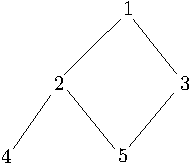
\includegraphics[width=30mm]{img/hasse5}
\end{center}

(a) Zapišite vse urejene pare, ki tvorijo relacijo $R$.

(b) Poiščite vse minimalne in maksimalne elemente.

(c) Ali ima množica $S$ prvi element? Ali ima množica $S$ zadnji element?

(d) Ali je množica $S$ dobro urejena?
\end{problem}

\textbf{Rešitev:}

(a) $R = \{(5,2),(5,1),(4,2),(4,1),(5,3),(4,1),(2,1),(3,1)\}$.

(b) Noben element ni pod elementoma 4 in 5, torej sta 4 in 5 minimalna elementa.
Maksimalen element pa je samo eden: 1.

(c) Množica $S$ nima prvega elementa. Elementa 4 in 5 sta sicer minimalna, vendar nobeden
od njiju ni pod drugim. Množica $S$ pa ima zadnji element: to je element 1, saj so vsi drugi elementi
pod njim.

(d) Ne, saj ni sovisna: Elementa 2 in 3 nista primerljiva: $(2,3)\not\in R$, $(3,2)\not\in R$.\qed

\bigskip
\textbf{Opomba:} \emph{Naj relacija $R$ strogo delno ureja množico $S$.
Tedaj je $x\in S$ minimalni element natanko tedaj, ko $x\not\in {\cal Z}R$.}

\emph{(${\cal Z}R$ = zaloga vrednosti relacije $R$ = množica vseh drugih koordinat).}

\emph{$x\in S$ pa je maksimalen element natanko tedaj, ko $x\not\in {\cal D}R$.}

\emph{(${\cal D}R$ = domena relacije $R$ = množica vseh prvih koordinat).}


\begin{enumerate}


\item Naj velja $S=\{1,2,3,4,5\}$. 
\begin{enumerate}
    \item Ali je  $R=\{(1,2),(2,3), (3,5), (2,4), (5,1)\}$ binarna relacija?
    \item Za relacijo $R$ najdi ustrezno domeno $\mathcal{D} R$, in zalogo vrednosti $\mathcal{Z} R$.
    \item 
  Določi inverzno relacijo $R^{-1}$ in  $\mathcal{D} R^{-1}$ in  $\mathcal{Z} R^{-1}$.
\end{enumerate}

\item Naj bosta $R=\{(1,1),(2,1), (3,3), (1,5)\}$  in $T=\{(1,4),(2,1), (2,2), (2,5)\}$ binarni relaciji v vesolju $S=\{1,2,3,4,5\}$. \begin{enumerate}
    \item 
Določi kompozituma  $R\circ T$ in $T\circ R$. 
\item Ali velja $R\circ T = T \circ R$?
\end{enumerate}

\item Naj velja  $S=\{1,2,3,4,5,6,7\}$. Določi
$$R= \{(x,y)\,|\, x-y \text{ je deljivo z  }  3\} \quad \mathrm{ in } \quad  T= \{(x,y)\,|\, x-y \geq 3\}.$$
Določi $R,T, R\circ R$.


\item V vesolju  $S= \mathbb{R}$  definiramo  relacijo $R$:
$$(\forall x)(\forall y)(x R y \Leftrightarrow y \geq x +3).$$
Je $R$ refleksivna, simetrična, tranzitivna, ali sovisna?

\item Naj velja  $S=\{1,2,3,4\}$. Imamo spodnje relacije:
\begin{enumerate}
\item[(i)] $R_1= \{(1,1),(1,2),(2,3), (1,3), (4,4)\}$,
\item[(ii)] $R_2= \{(1,1),(1,2),(2,1), (2,2), (3,3), (4,4)\}$,
\item[(iii)] $R_3= \{(1,3),(2,1)\}$,
\item[(iv)] $R_4= \emptyset$,
\item[(v)] $R_5= S\times S$.
\end{enumerate}
Za katere od naštetih relacij velja, da so: refleksivne, simetrične, antisimetrične, tranzitivne? 

\item Naj bosta $R$ in $S$ simetrični relaciji. Pokaži: $R\circ S$ simetrična $\Leftrightarrow R\circ S = S \circ R$.


	\item Naj bo $S=\{ (x,y) \,:\, x, y\in\mathbb{R} \textrm{ in } y\leq 0 \}$ in naj bo $R$ relacija na množici $S$, definirana kot 
	$$(x_1,y_1)\, R\, (x_2,y_2) \Leftrightarrow  x_1 = x_2 \textrm{ in } y_1\leq y_2.$$
	\begin{enumerate}
		\item[(i)] Dokažite, da je $R$ delna urejenost na $S$.
		\item[(ii)] Najdite vse $R$-minimalne elemente.
	\end{enumerate}
	
	\item Naj bo $S= \{0,\frac{1}{2}, \frac{2}{3}, \frac{3}{4}, \ldots, \frac{n}{n+1}, \ldots, 1\}$, in naj bo $R:=<$ relacija na $S$. Ali $R$ dobro ureja $S$?
	
	\item Naj bo $S = \mathbb{N}\setminus \{0\}$ in naj bo  $R$ relacija na $S$, definirana kot 
	$$m\, R\, n \Leftrightarrow  \textrm{ $p< u$ ali ($p=u$ in $q < v$),} $$
	kjer je $m=2^p(2q+1)$ in $n=2^u(2v+1)$, pri čemer sta $p$ in $u$ maksimalno možna eksponenta.
	\begin{enumerate}
		\item[(i)] Dokažite, da $R$ dobro ureja $S$.
		\item[(ii)] Uredite množico $\{1,2\ldots, 10\}$ glede na $R$.
		\item[(iii)] Naj bo $C= \{50, 51, 52, \ldots\}$. Najdite $R$-minimalni element množice $C$.
		\item[(iv)] Najdite neposrednega naslednika števila $96$.
	\end{enumerate}
\end{enumerate}

\section{Ekvivalenčne relacije}

\begin{enumerate}
  \item \textbf{Zgled: Ulomki.}

  V množici ulomkov $$a/b\,,$$
  kjer sta $a$ in $b$ poljubni celi števili in je $b\neq 0$, je definicija enakosti dveh ulomkov
  $$a/b = c/d \cee ad = bc$$
  očitno ekvivalenčna relacija. Vsak ekvivalenčni razred glede na to relacijo druži vse med seboj enake ulomke in predstavlja tedaj ustrezno {\em racionalno število}. Prirejena faktorska množica je {\em množica racionalnih števil}.
  \item \textbf{ Kongruence.}


  V množici {\em celih števil} je relacija {\em kongruence po modulu $m$}, kjer je $m> 0$ poljubno pozitivno celo število, $$a\equiv b \textrm{ (mod $m$)}\cee m \textrm{ deli }a-b\,,$$
  ekvivalenčna relacija.

  Ekvivalenčni razredi so v tem primeru {\em razredi ostankov} po modulu $m$. V vsakem ekvivalenčnem razredu so vsa tista števila, ki dajo pri deljenju z $m$ isti ostanek.

  Očitno je takih razredov natanko $m$. Te razrede imenujemo {\em cela števila po modulu $m$}. Faktorska množica je množica celih števil po modulu $m$.

  \item \textbf{Zgled: Vzporednost premic.}

V množici {\em vseh premic} je relacija ``vzporeden'' ekvivalenčna relacija. V vsakem ekvivalenčnem razredu so torej vse premice, ki so med seboj vzporedne, in predstavljajo potemtakem določeno {\em smer}. Faktorska množica je tukaj {\em množica vseh smeri}.



\item Let $S= \{m\in \mathbb{N}\,|\, 1\leq n \leq 10\}$ in $R=\{(m,n)\in S\times S\,|\, 3|m-n\}$.
Is $R$ an equivalence relation? If yes, determine the corresponding equivalence classes and the factor set.

\item Let $S = \mathbb{Z}\times \mathbb{Z}$ and define the relation $R$ as follows
$$(a,b)R(c,d)\Leftrightarrow ad = bc.$$
Show that $R$ is an equivalence relation  and find the corresponding equivalence classes.

\item Let  $S =  \mathbb{R}^2$ and define the relation $R$ as follows
$$(x_1,y_1)R(x_2,y_2)\Leftrightarrow x_1^2 + y_1^2 = x_2^2 + y_2^2.$$
Show that $R$ is an equivalence relation  and find the equivalenece class $R[(7,1)]$.

\end{enumerate}




\section{Grafi}
\begin{enumerate}
\item Naj velja $n\ge 3$. Spomnimo definicijo ciklov in polnih grafov
\[C_{n}=\{[n], E_{1}\}\]
\[K_{n}=\{[n], E_{2}\}\]
ter definirajmo 
\[G_{n}=\{[n], E_{2} \setminus E_{1}\}\]
\begin{itemize}
    \item Nariši \(H, G_{4}, G_{5}, G_{6}, C_{5}, C_{6}, \overline{C_{i}}\)
    \item Za  vse zgornje grafe določi \(\Delta(G_{i}), \delta(G_{i}), \alpha(G_{i}), \omega(G_{i}), \chi(G_{i}), g(G_{i})\)
    \item
Dokaži \((\forall i \geq 3) (G_{i} \simeq \overline{C_{i}})\)
\end{itemize}


\item
Naj bo \(G = ([n], E)\) graf.
\begin{itemize}
\item
Dokaži: \(\chi (G) \geq \omega (G)\)

\item
Dokaži: \(\chi (G) \geq \frac{n}{\alpha(G)}\)
\end{itemize}

\end{enumerate}

\chapter{Končne in neskončne množice}

\section{Pregled najpomembnejših pojmov in nekaj nalog}

Ključni pojmi:
\begin{itemize}
\item Relacija ekvipolence: $A\sim B$.
%\item Ekvipolentna relacija je ekvivalenčna relacija.
\item Relacija $>$ na množicah (``ima večjo moč kot").
%\item 4 logične možnosti.
\item Schröder-Bernsteinov izrek: Množici $A$ in $B$ sta ekvipolentni, če je vsaka od
njiju ekvipolentna neki podmnožici druge.
\item Zakon trihotomije.
\item Definicije končnih in neskončnih množic. (S pomočjo $\mathbb N$; Peirce-Dedekind; Tarski.)
%\item Lastnosti končnih množic.
%\item Lastnosti neskončnih množic.
\item Množica $\mathbb N$, Peanovi aksiomi.
\item Števno neskončne množice.
\item Interval $(0,1]$ ni števno neskončna množica; Cantorjev dokaz.
\item $(0,1]\sim [0,1)\sim [0,1]\sim (0,1)\sim (-1,1)\sim \mathbb{R}$.
\item Kontinuum. $\mathbb{R}>\mathbb{N}$.
\item Cantorjev izrek. Domneva kontinuuma.
\end{itemize}

\begin{problem}
Pokažite, da ima množica vseh funkcij
$\{f:\mathbb{R}\to \mathbb{R}\}$ večjo moč kot $\mathbb{R}$.
\end{problem}


\bigskip
\textbf{Rešitev:} Pokazali smo, da je potenčna množica poljubne množice $X$
ekvipolentna množici ${\cal C}(X)$ vseh funkcij $f:X\to \{0,1\}$.
Po Cantorjevem izreku je torej
$${\cal C}(\mathbb{R})\sim {\cal P}(\mathbb{R})>\mathbb{R}\,.$$
Torej ima že množica vseh funkcij $f:\mathbb{R}\to \{0,1\}$ večjo moč od kontinuuma!
\qed


\section{Zgledi števno neskončnih množic}

\bigskip
{\em Množica celih števil} $\mathbb{Z}$ je števno neskončna (saj je $\mathbb{Z} = \mathbb{N}\cup (-\mathbb{N})$).

\bigskip
\hrule
\bigskip

Tudi {\em množica racionalnih števil} $\mathbb{Q}$ je števno neskončna!

Očitno je dovolj pokazati, da je množica pozitivnih racionalnih števil $\mathbb{Q}_+$
 števno neskončna, saj je $\mathbb{Q} = \mathbb{Q}_-\cup \{0\}\cup \mathbb{Q}_+$ in je
$\mathbb{Q}_-\sim \mathbb{Q}_+$.

Množico $\mathbb{Q}_+$ pa lahko zapišemo kot števno unijo števno neskončnih množic:
$$\mathbb{Q}_+ = A_1\cup A_2\cup \cdots$$
kjer je:

$A_1 = \{\frac{1}{1}, \frac{2}{1}, \frac{3}{1}, \ldots\}$,

$A_2 = \{\frac{1}{2}, \frac{2}{2}, \frac{3}{2}, \ldots\}$,

$A_3 = \{\frac{1}{3}, \frac{2}{3}, \frac{3}{3}, \ldots\}$, $\ldots$

%\bigskip
%$-----------------$
%\bigskip

{\em Algebraično število}: tako kompleksno število $x$, ki je rešitev kake enačbe oblike
$$a_nx^n+a_{n-1}x^{n-1}+\ldots+a_1x+a_0 = 0\,,$$
kjer je $n\in \mathbb{N}$, $n\neq 0$, $a_n\neq 0$ in $a_i\in \mathbb{Z}$ za vse $i$.
Tudi množica algebraičnih števil je števno neskončna. Zapišemo jo namreč lahko kot
(števno neskončno) unijo končnih množic:
$$A_1\cup A_2\cup A_3\cup \cdots\,,$$
kjer je $A_k$ množica vseh kompleksnih števil, ki so rešitve
kakšne enačbe zgornje oblike, pri čemer za njene koeficiente velja
$n+|a_0|+|a_1|+\ldots+|a_n|\le k$.
Vsaka množica $A_k$ je končna, saj vsebuje le ničle kvečjemu
$(2k+1)^{k+1}$ polinomov stopnje $\le k$ s koeficienti iz množice $\{-k,-(k-1), \ldots, k-1,k\}$, vsak od takih polinomov pa ima
$\le k$ ničel.



%Da se prepričamo, da velja
%$$\mathbb{R}>\mathbb{N}\,,$$
%je dovolj pokazati, da obstaja podmnožica $X$ realnih števil, ekvipolentna množici
%${\cal P}(\mathbb N)$. Tedaj bo po Cantorjevem izreku $$\mathbb{R}\gtrsim X\sim {\cal P}(\mathbb N)>\mathbb{N}\,.$$
%
%Definirajmo funkcijo $f:{\cal P}(\mathbb N)\to [0,1)$ s predpisom:
%$$f(S) = 0,a_0a_1a_2a_3\ldots\,,$$
%kjer je
%$$a_i = \left\{
%        \begin{array}{ll}
%          1, & \hbox{če je $i\in S$;} \\
%          0, & \hbox{sicer.}
%        \end{array}
%      \right.$$
%Ta funkcija je očitno injektivna. Torej lahko za iskano množico $S$ vzamemo zalogo vrednosti ${\cal Z}f = f({\cal P}(\mathbb{N}))$.
%
%\medskip
%Velja celo ${\cal P}(\mathbb N)\sim \mathbb{R}$.

%\newpage
%\subsection*{Za vaje}
%
%\begin{trditev}
%Aksiom izbire $\cee$ Vsaka binarna relacija vsebuje funkcijo z isto domeno.
%\end{trditev}
%
%\begin{proof}
%$(\Rightarrow)$:
%
%Naj bo $R$ binarna relacija na množici $S$ in naj bo $I={\cal D}R$ domena te relacije.
%
%Za $\lambda \in I$ definirajmo množico
%$$A_\lambda = \{a~;~a\in S\inn \lambda Ra\}\,.$$
%
%${\cal A} = \{A_\lambda~;~\lambda \in I\}$ je potemtakem družina nepraznih množic.
%Aksiom izbire zagotavlja obstoj funkcije $f:I\to \cup A_\lambda$, za katero velja
%$f(\lambda)\in A_{\lambda}$ za vse $\lambda\in I$.
%Torej je $\lambda Rf(\lambda)$ za vse $\lambda\in I$ in je $f$ funkcija, vsebovana
%v relaciji $R$. Domena funkcije $f$ pa je seveda $I = {\cal D}R$.
%
%\medskip
%($\Leftarrow$):
%
%Naj bo ${\cal A} = \{A_\lambda~;~\lambda \in I\}$ družina nepraznih množic.
%
%Definirajmo binarno relacijo $R$ na množici $$I\cup (\cup {\cal A})$$
%na naslednji način:
%$$R = \{(\lambda,x)~;~\lambda\in I\inn x\in A_\lambda\}\,.$$
%Po predpostavki obstaja neka funkcija $f$, vsebovana v $R$, katere domena je
%${\cal D}R = I$.
%Za vsak $\lambda\in I$ torej velja $(\lambda, f(\lambda))\in R$, tj., $f(\lambda)\in A_\lambda$.
%Torej je $f$ funkcija izbire.
%\end{proof}
%
%Trditev  \emph{ ``Vsaka binarna relacija vsebuje funkcijo z isto domeno."~}
%je moč izpeljati tudi direktno iz Zornove leme. Dokaz te implikacije (ki ga opustimo)
%temelji na naslednji trditvi o funkcijah:
%
%\begin{trditev}
%Naj bo množica funkcij $\{f_i:A_i\to B~;~i\in I\}$ linearno urejena glede na inkluzijo $\subseteq$. Potem je unija $\cup_{i\in I}f_i$ funkcija iz $\cup_{i\in I}A_i$ v $B$.
%\end{trditev}
%
%\begin{proof}
%Naj bo $f = \cup_{i\in I}f_i$. Domena te relacije je
%množica vseh prvih koordinat, torej očitno unija vseh domen funkcij
%$f_i$:  $${\cal D}f = \cup_{i\in I}{\cal D}f_i
%= \cup_{i\in I}A_i\,.$$
%Množica vseh drugih koordinat je prav tako unija vseh
%množic drugih koordinat, torej podmnožica množice $B$.
%
%$f$ je res funkcija:
%
%Recimo, da je $(x,y)\in f$ in $(x,z)\in f$.
%Tedaj obstaja tak $i\in I$, da je $(x,y)\in f_i$, torej
%$x\in A_i$ in $y = f_i(x)$.
%Prav tako obstaja tak $j\in I$, da je $(x,z)\in f_j$, torej
%$x\in A_j$ in $z = f_j(x)$.
%
%Po predpostavki o linearni urejenosti je bodisi
%$f_i\subseteq f_j$ bodisi $f_j\subseteq f_i$.
%Recimo, da je $f_i\subseteq f_j$. Tedaj je $(x,y)\in f_j$, torej
%$x\in A_j$ in $y = f_j(x)$.
%Tedaj pa je $y=z$. Če je $f_j\subseteq f_i$, pa je $z = f_i(x) = y$.
%\end{proof}
%
%\begin{trditev}
%Aksiom izbire $\cee$
%Za vsako družino ${\cal A}$ paroma disjunktnih nepraznih množic obstaja taka
%množica $X$, da za vsak $A\in {\cal A}$ množica $X\cap A$ vsebuje natanko en element.
%\end{trditev}
%
%\begin{proof}
%$(\Rightarrow)$:
%
%Naj bo ${\cal A} = \{A_\lambda~;~\lambda\in I\}$ družina paroma disjunktnih nepraznih množic.
%Po aksiomu izbire obstaja taka funkcija $f:I\to \cup {\cal A}$, da
%za vse $\lambda \in I$ velja $f(\lambda)\in A_\lambda$.
%Definirajmo $X = \textrm{Im} f$, zaloga vrednosti funkcije $f$.
%Tedaj je $X$ iskana množica, saj za vsak $\lambda\in I$ velja
%$X\cap A_\lambda = \{f(\lambda)\}$:
%\begin{itemize}
%  \item očitno je $f(\lambda)\in X\cap A_\lambda$;
%  \item če je $y\in X\cap A_\lambda$ potem obstaja tak $\mu \in I$, da
%  velja $y = f(\mu)$, ker pa je $x\in A_\lambda$ in so
%  množice $\{A_\lambda~;~\lambda\in I\}$ paroma disjunktne, je
%  $\mu = \lambda$ in zato $y = f(\lambda)$.
%\end{itemize}
%
%\medskip
%($\Leftarrow$):
%
%Naj bo ${\cal A} = \{A_\lambda~;~\lambda \in I\}$ družina nepraznih množic.
%
%Definirajmo družino množic $$\{B_\lambda~;~\lambda\in I\}$$
%s predpisom
%$$B_\lambda = \{\lambda\}\times A_\lambda$$
%za vse $\lambda\in I$.
%Množice $B_\lambda$ so vse neprazne. So pa tudi paroma disjunktne:
%
%Recimo, da je $B_\lambda\cap B_\mu \neq\emptyset$ in naj
%bo $(x,y)\in B_\lambda\cap B_\mu$.
%Potem je $x = \lambda$ (ker je $(x,y)\in B_\lambda$) in tudi $x = \mu$ (ker je $(x,y)\in B_\mu$).
%Sledi $\lambda = \mu$.
%
%Po predpostavki obstaja taka množica $X$, da za vsak $\lambda \in I$ množica $X\cap B_\lambda$ vsebuje natanko en element,
%recimo mu $(\lambda, x_\lambda)$. Ker je $(\lambda, x_\lambda)\in B_\lambda$, je
%$x_\lambda\in A_\lambda$. Funkcija izbire $f:I\to \cup {\cal A}$ torej obstaja: definirana je s predpisom
%$f(\lambda) = x_\lambda$ za vse $\lambda\in I$.
%\end{proof}
%
%
%\bigskip
%
%Spomnimo se, da s simbolom $A^B$ označujemo množico vseh funkcij iz množice $B$ v množico $A$.
%
%  $A\sim C$ in $B\sim D$ $\sledi$ $A^B\sim C^D$.
%
%Naj bosta $g:A\to C$ in $h:B\to D$ bijekciji. Konstruiramo naslednjo preslikavo:
%
%$$A^B\to C^D$$
%
%$$f\mapsto f' = g\circ f\circ h^{-1}\,.$$
%
%Tedaj je $f'=g\circ f\circ h^{-1}:D\to C$,
%
%$f'(x) = g(f(h^{-1}(x)))$.
%
%Prepričajmo se, da je preslikava $f\mapsto f'$ bijektivna.
%
%\begin{itemize}
%  \item injektivnost:
%
%  Recimo, da je $g\circ f_1\circ h^{-1} = g\circ f_2\circ h^{-1}$.
%
%  Pokazati moramo: $f_1(x) = f_2(x)$ za vse $x\in B$.
%
%  Vzemimo poljuben $x\in B$ in si oglejmo element $y = h(x)$. Vemo, da ga funkciji $g\circ f_1\circ h^{-1}$ in $g\circ f_2\circ h^{-1}$
%  preslikata v isti element, saj sta enaki.
%  Torej: $g(f_1(h^{-1}(h(x)))) =  g(f_2(h^{-1}(h(x))))$ $\sledi$ $g(f_1(x)) = g(f_2(x))$.
%  Torej tudi $g^{-1}(g(f_1(x))) = g^{-1}(g(f_2(x)))$. Sledi $f_1(x) = f_2(x)$.
%
%  \item surjektivnost:
%
%  Naj bo $F:D\to C$ poljubna funkcija. Iščemo tak $f:B\to A$, da bo veljalo $g\circ f\circ h^{-1} = F$.
%
%  Torej $f\circ h^{-1} = g^{-1}\circ F$ in posledično  $f= g^{-1}\circ F\circ h$.
%  $F$ je torej slika elementa $g^{-1}\circ F\circ h$.
%  \end{itemize}




\end{document}

